\documentclass{article}

\usepackage{graphicx}
\usepackage{amsmath}
\usepackage{hyperref}

\title{Does Anonymity Inflate the Subject?\\
A Comparative LLM-Based Analysis of Political and 4chan Discourse}

% 著者情報を削除
%\author{Nazuki Takahashi}

\date{}

\begin{document}

\maketitle

\begin{abstract}
This study analyzes subject size in online posts using a 
large language model and compares subject sizes 
between posts written by identified politicians and anonymous 4chan users. 
The study investigates whether anonymous users employ larger subjects, as 
criticized by Schopenhauer. The statistical results show a statistically 
significant difference between the two groups (politicians: 2.10, 4chan: 2.18). 
However, the effect size is small, suggesting that anonymity does not strongly 
affect subject size in online communication.
\end{abstract}

\noindent
\textbf{Keywords:} online anonymity, subject abstraction, large language model, 4chan, political communication

\section{Introduction}

\begin{quote}
``A particularly ludicrous impertinence of such anonymous critics is that they,
like kings, speak in the first-person plural `we'; whereas they should speak
not in the plural we but, at most, in the singular.'' (Schopenhauer, 1851)
\end{quote}

Schopenhauer criticizes anonymous writers for their use of the 
first-person plural ``we,'' arguing that such usage falsely projects authority 
and collective legitimacy. Anonymous authors tend to use the first-person plural 
rather than the singular form.

Numerous studies suggest anonymity increases toxicity and behavioral 
disinhibition. Suler (2004) shows that people self-disclose or act out more 
frequently or intensely online. Nitschinsk et al.\ (2023) show that one motivation 
for being online is to seek anonymity for self-expression or toxic behavior.

\section{Methods}

\subsection{Data}

To score subject sizes, we used the dataset \textit{Social Media Posts from US 
Politicians} (Damarla, 2020), consisting of approximately 5000 posts. 
For 4chan posts, we collected approximately 5000 posts from the /pol/ subforum.

4chan data contains raw HTML and platform-specific syntax (e.g., greentext 
or post citations). A Python script was used to clean and normalize the text. 
The script removed HTML tags, converted character entities, and stripped 
post-ID references to ensure data consistency. The scripts are available upon request for reproducibility.

\subsection{Subject Scale}

Four stages of subject abstraction were defined:

\begin{enumerate}
\item \textbf{Singular} – an individual, clearly identifiable entity (e.g., I, you, he, she, a named person).
\item \textbf{Plural} – a clear collection of individuals (e.g., we, they, teachers).
\item \textbf{Collective} – an organizational or institutional entity treated as a single subject (e.g., government, company, university).
\item \textbf{Concept} – highly generalized or conceptual entities (e.g., society, humanity, the nation).
\end{enumerate}

\subsection{LLM Analysis}

To scale subject size automatically, we used a large language model executed locally using llama.cpp. 
A zero-shot prompt was used to isolate the ``size'' of the subject 
independently from emotional tone or sentiment.

\begin{itemize}
\item n\_predict: 400
\item temperature: 0.4
\item top\_k: 40
\item top\_p: 0.95
\item repeat\_penalty: 1.18
\end{itemize}

\subsection{Statistical Tests}

Welch's t-test and Kolmogorov–Smirnov test were used to compare subject sizes. 
Cohen's $d$ measured effect size ($\alpha = 0.05$). Scripts used for analysis 
are available upon request.

\section{Results}

Posts by US politicians had a mean subject size of 2.10 ($SD = 1.01$), 
median 1.7. 4chan /pol/ posts had mean 2.18 ($SD = 0.99$), median 2.0.

\begin{table}[h]
\centering
\begin{tabular}{lcccccc}
\hline
Dataset & N & Mean & Median & Std. Dev & Min & Max \\
\hline
US Politicians & 4733 & 2.10 & 1.7 & 1.01 & 1.0 & 4.5 \\
4chan /pol/ & 4960 & 2.18 & 2.0 & 0.99 & 1.0 & 4.5 \\
\hline
\end{tabular}
\caption{Subject size statistics for the two datasets}
\end{table}

\begin{figure}[h]
\centering
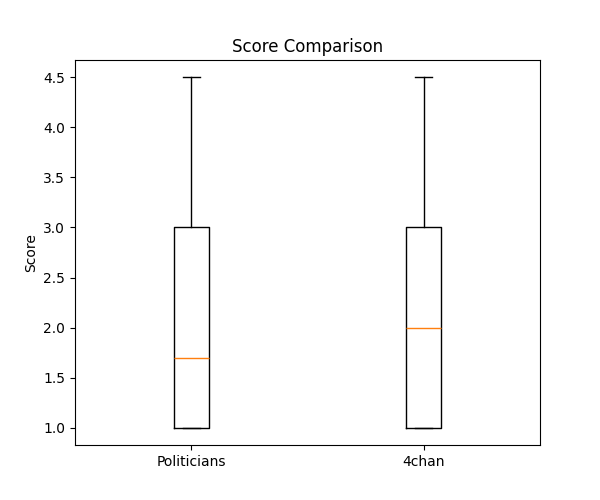
\includegraphics[width=0.7\linewidth]{imgs/Figure_2.png}
\caption{Boxplot comparison of subject size between posts by US politicians and 4chan /pol/ users.}
\end{figure}

\begin{figure}[h]
\centering
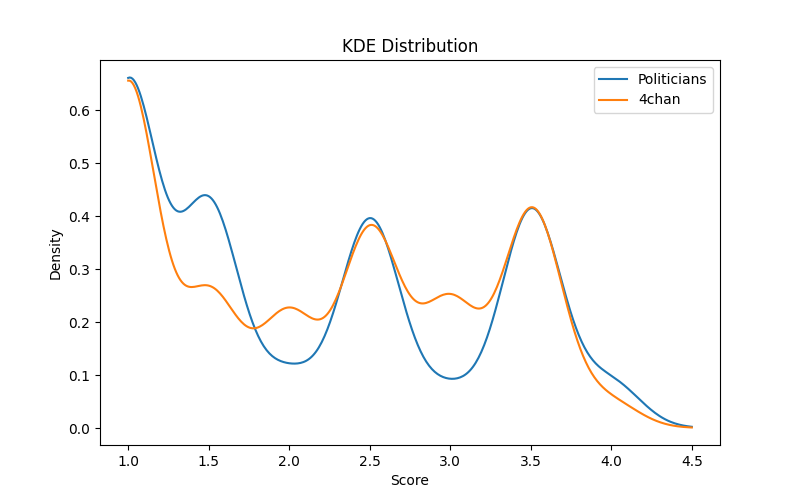
\includegraphics[width=0.7\linewidth]{imgs/Figure_6.png}
\caption{Kernel density estimation (KDE) of subject size distributions for the two datasets.}
\end{figure}

\begin{figure}[h]
\centering
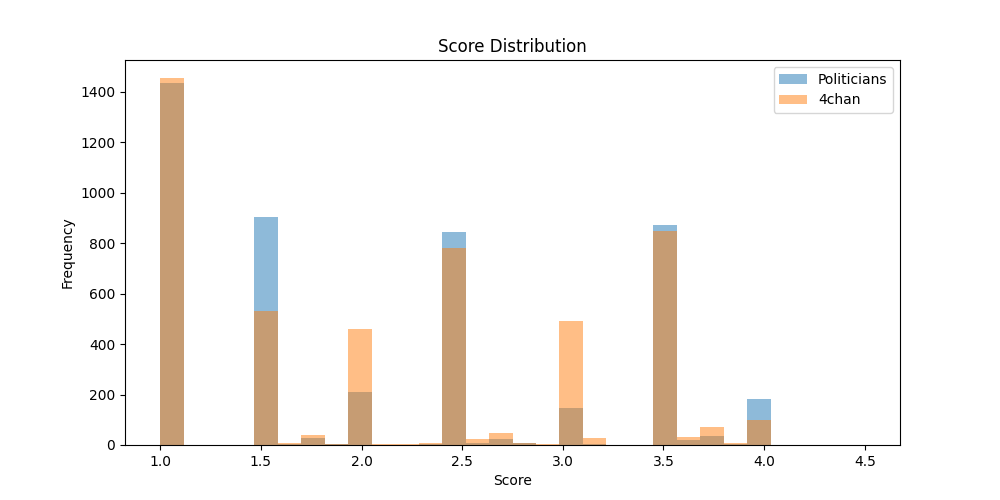
\includegraphics[width=0.7\linewidth]{imgs/Figure_1.png}
\caption{Histogram of subject size distributions for posts by US politicians and 4chan /pol/ users.}
\end{figure}

\begin{figure}[h]
\centering
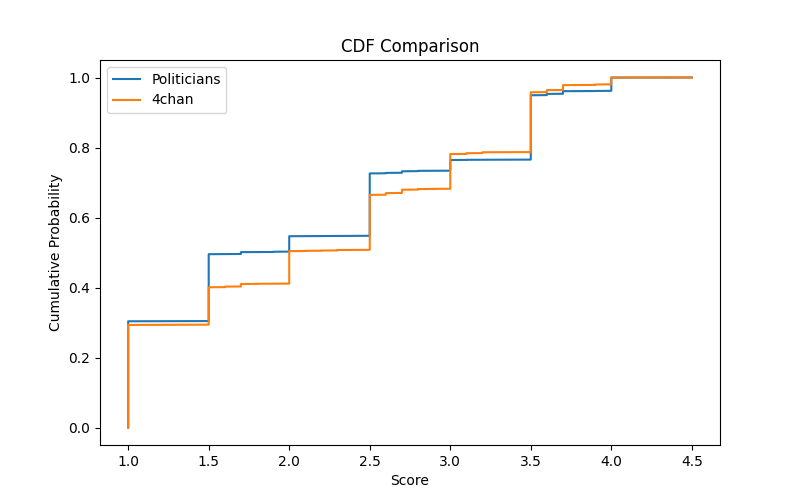
\includegraphics[width=0.7\linewidth]{imgs/Figure_4.png}
\caption{Cumulative distribution function (CDF) comparison of subject size distributions.}
\end{figure}

Welch's t-test indicated statistically significant differences ($t = -4.04$, $p < 0.001$), 
but small effect size (Cohen's $d = -0.082$). KS test also significant ($D = 0.094$, $p < 0.001$).

\section{Discussion}

Posts on 4chan /pol/ exhibit slightly higher mean subject size. Although statistically significant, the small effect size suggests anonymity does not dramatically inflate subject abstraction.

Anonymous users discuss broad social categories (``they,'' ``the people''), slightly increasing abstraction. Politicians also use collective subjects (``our government,'' ``our nation''), reducing differences. High overlap suggests online discourse encourages collective framing regardless of anonymity.

\subsection{Limitations and Future Research}

\begin{itemize}
\item Platform differences
\item Topic differences
\item Limitations of subject scale definition
\end{itemize}

Future work should separate grammatical person (``we'') from conceptual abstraction and expand to other platforms such as Reddit.

\section{Conclusion}

Anonymity alone does not substantially change subject framing online. Both identified and anonymous speakers rely on similar ranges of subject abstraction.

\begin{thebibliography}{9}

\bibitem{damarla2020}
Damarla, R. (2020). \textit{Social Media Posts from US Politicians}. Kaggle dataset.

\bibitem{nitschinsk2023}
Nitschinsk, J., et al. (2023). Online anonymity and behavioral expression. \textit{Procedia Computer Science}.

\bibitem{schopenhauer1851}
Schopenhauer, A. (1851). \textit{Parerga and Paralipomena}.

\bibitem{suler2004}
Suler, J. (2004). The online disinhibition effect. \textit{CyberPsychology \& Behavior}, 7(3), 321–326.

% GitHub リンクは匿名用では削除
%\bibitem{takahashi2026}
%Takahashi, N. (2026). Subject abstraction analysis code and data collection scripts. GitHub repository. 

\end{thebibliography}

\appendix

\section{LLM Prompt Used for Subject Size Evaluation}

\begin{verbatim}
Please rate the "subject size" of the post using the following criteria.
Only return a float number (e.g. 1.0, 2.3, 3.1). The number must include
a decimal. Output as a continuous value between 1.0 and 4.0.

Scale definition:

1.0 Singular
2.0 Plural
3.0 Collective
4.0 Concept

Pay attention only to the size of the subject.
Do not consider the emotional tone or content of the sentence.
\end{verbatim}

\end{document}